\section*{Appendix}

\begin{frame}{Training Hyperparameters}
	\centering
	\scriptsize
	\begin{threeparttable}
		\begin{tabular}{llc}
			\toprule
			\textbf{Model}           & \textbf{Hyperparameter} & \textbf{Value}   \\
			\midrule
			\multirow{7}{*}{RF-DETR} & LR decoder              & \num{1e-4}       \\
			                         & LR backbone             & \num{1.5e-4}     \\
			                         & Drop path rate          & 0.1              \\
			                         & Batch size              & 16               \\
			                         & Optimizer               & AdamW            \\
			                         & Warmup epochs           & 5                \\
			                         & Resolution (px)         & $512 \times 512$ \\
			\midrule
			\multirow{5}{*}{YOLO26}  & LR                      & \num{1e-4}       \\
			                         & Batch size              & 16               \\
			                         & Resolution (px)         & $640 \times 640$ \\
			                         & Optimizer               & AdamW            \\
			                         & Warmup epochs           & 10               \\
			\bottomrule
		\end{tabular}
		\begin{tablenotes}
			\tiny{
				\item Training and inference on all models and variants done in resolution native to respective architectures
			}
		\end{tablenotes}
	\end{threeparttable}
\end{frame}

\begin{frame}{Full Scaling Study}
	\centering
	\scriptsize
	\setlength{\tabcolsep}{4pt}
	\begin{tabular}{llccccc}
		\toprule
		\textbf{Model}           & \textbf{Var.} & \textbf{\mapfn} & \textbf{\mapf}  & \textbf{Pre}    & \textbf{Rec}    & \textbf{F1}     \\
		\midrule
		\multirow{5}{*}{RF-DETR} & X-Large       & 0.5043          & 0.8301          & 0.8034          & 0.7588          & 0.7799          \\
		                         & Large         & \textbf{0.5249} & \textbf{0.8430} & 0.7903          & \textbf{0.7927} & \textbf{0.7911} \\
		                         & Medium        & 0.5007          & 0.8231          & 0.8195          & 0.7519          & 0.7839          \\
		                         & Small         & 0.4829          & 0.8202          & \textbf{0.8562} & 0.7104          & 0.7758          \\
		                         & Nano          & 0.4153          & 0.7659          & 0.8222          & 0.6825          & 0.7446          \\
		\midrule
		\multirow{5}{*}{YOLO26}  & X-Large       & 0.5060          & \textbf{0.8067} & 0.7983          & 0.7387          & \textbf{0.7673} \\
		                         & Large         & 0.4957          & 0.8016          & 0.7827          & \textbf{0.7435} & 0.7625          \\
		                         & Medium        & \textbf{0.5069} & 0.8027          & \textbf{0.8104} & 0.7082          & 0.7557          \\
		                         & Small         & 0.4918          & 0.7915          & 0.8090          & 0.7180          & 0.7614          \\
		                         & Nano          & 0.4540          & 0.7643          & 0.7892          & 0.6700          & 0.7240          \\
		\bottomrule
	\end{tabular}
\end{frame}

\begin{frame}{Full Deployment Profile}
	\centering
	\scriptsize
	\setlength{\tabcolsep}{4pt}
	\begin{tabular}{llcccc}
		\toprule
		\textbf{Model} & \textbf{Variant} & \textbf{FPS} & \textbf{Lat.\ (ms)} & \textbf{Mem.\ (MB)} & \textbf{Pow.\ (W)} \\
		\midrule
		\multirow{5}{*}{YOLO26}
		               & Nano             & \textbf{285} & \textbf{3.5}        & 46                  & 62                 \\
		               & Small            & 282          & 3.5                 & 66                  & 62                 \\
		               & Medium           & 213          & 4.7                 & 102                 & 62                 \\
		               & Large            & 165          & 6.0                 & 113                 & 64                 \\
		               & X-Large          & 121          & 8.3                 & 194                 & 66                 \\
		\midrule
		\multirow{5}{*}{RF-DETR}
		               & Nano             & 44           & 22.6                & 207                 & 57                 \\
		               & Small            & 46           & 21.9                & 211                 & 65                 \\
		               & Medium           & 46           & 21.6                & 219                 & 58                 \\
		               & Large            & 46           & 21.7                & 220                 & 64                 \\
		               & X-Large          & 36           & 27.5                & 607                 & 84                 \\
		\bottomrule
	\end{tabular}
\end{frame}

\begin{frame}{Full Class-wise AP}
	\centering
	\scriptsize
	\setlength{\tabcolsep}{5pt}
	\begin{tabular}{llccc}
		\toprule
		\textbf{Model} & \textbf{Variant} & \textbf{Bottle} & \textbf{Bag}    & \textbf{Can}    \\
		\midrule
		\multirow{5}{*}{RF-DETR}
		               & X-Large          & 0.5769          & 0.3735          & 0.5028          \\
		               & Large            & \textbf{0.6189} & \textbf{0.4102} & \textbf{0.5458} \\
		               & Medium           & 0.5891          & 0.3867          & 0.5265          \\
		               & Small            & 0.5654          & 0.3819          & 0.4919          \\
		               & Nano             & 0.5325          & 0.3515          & 0.4605          \\
		\midrule
		\multirow{5}{*}{YOLO26}
		               & X-Large          & 0.6130          & \textbf{0.4010} & \textbf{0.5420} \\
		               & Large            & 0.6020          & 0.3800          & 0.5070          \\
		               & Medium           & \textbf{0.6210} & 0.3870          & 0.5370          \\
		               & Small            & 0.6070          & 0.3730          & 0.5330          \\
		               & Nano             & 0.4892          & 0.3320          & 0.4208          \\
		\bottomrule
	\end{tabular}
\end{frame}

\begin{frame}{Extra Cases (1/2)}
	\begin{center}
		\begin{tabular*}{0.9\linewidth}{@{\extracolsep{\fill}}ccc@{}}
			\scriptsize\textbf{Ground Truth} & \scriptsize\textbf{YOLO26} & \scriptsize\textbf{RF-DETR} \\
		\end{tabular*}
		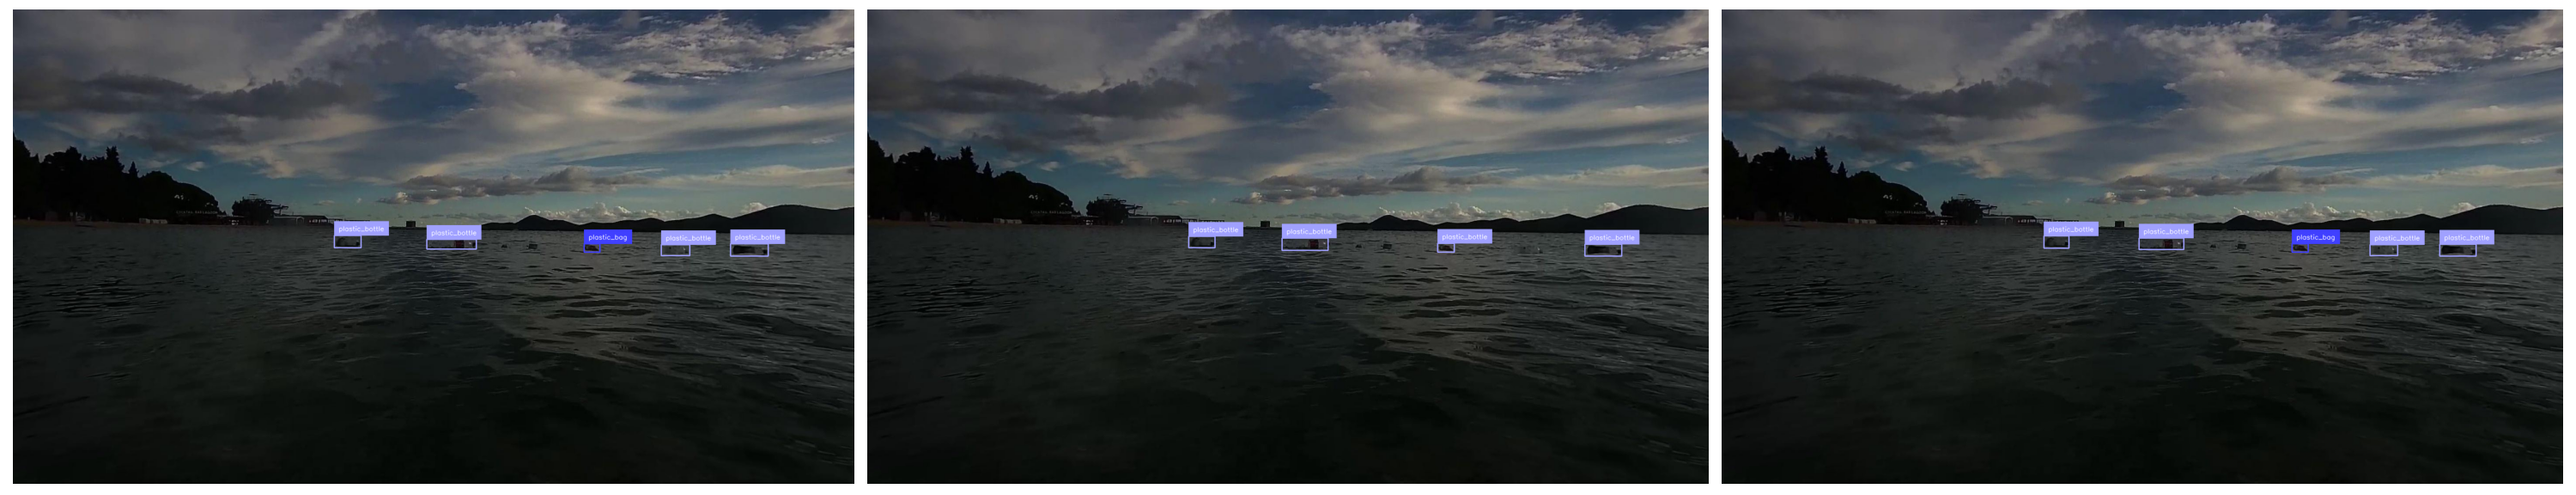
\includegraphics[width=0.95\linewidth]{figures/yolo26-bag-miss.png} \\
		{\tiny Dusk, low contrast: YOLO26 mislabels plastic bag, RF-DETR identifies all correctly.}
	\end{center}
\end{frame}

\begin{frame}{Extra Cases (2/2)}
	\begin{center}
		\begin{tabular*}{0.9\linewidth}{@{\extracolsep{\fill}}ccc@{}}
			\scriptsize\textbf{Ground Truth} & \scriptsize\textbf{YOLO26} & \scriptsize\textbf{RF-DETR} \\
		\end{tabular*}
		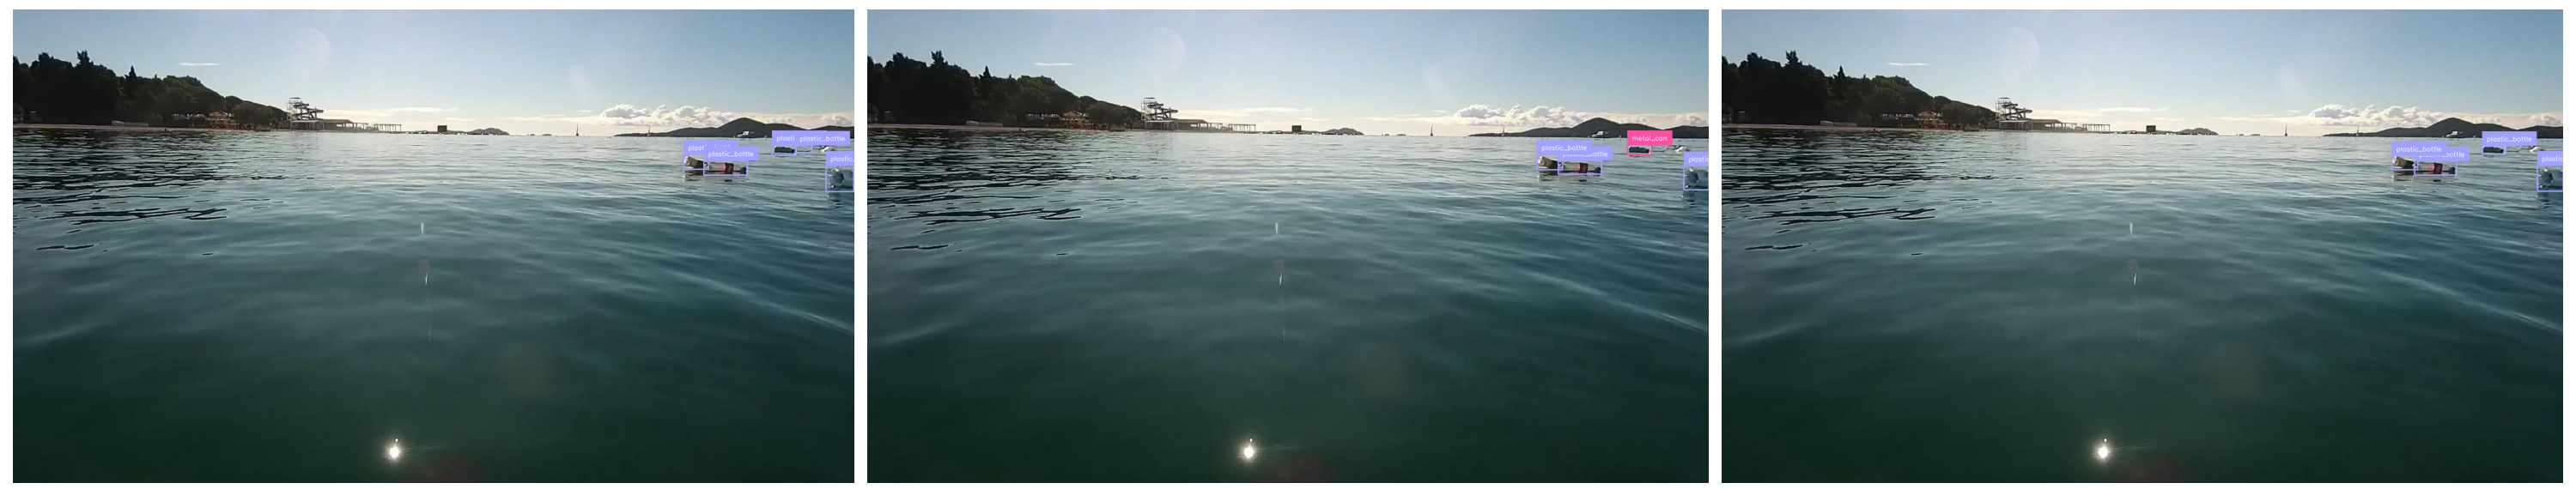
\includegraphics[width=0.95\linewidth]{figures/yolo26-mislabel.png} \\
		{\tiny YOLO26 mislabels debris; RF-DETR matches ground truth.}
	\end{center}
\end{frame}

\begin{frame}{Metrics Primer}
	\begin{columns}[T]
		\begin{column}{0.47\textwidth}
			\begin{itemize}
				\item Precision: correct over predicted
				\item Recall: found over total
				\item F1 balances both scores
			\end{itemize}
		\end{column}
		\begin{column}{0.49\textwidth}
			\begin{block}{\mapf\ vs \mapfn}
				\begin{equation*}
					\text{mAP} = \frac{1}{C}\sum_c AP_c
				\end{equation*}
				\mapf: IoU 0.50. \mapfn: mean over 0.50--0.95.
			\end{block}
		\end{column}
	\end{columns}
\end{frame}

% \begin{frame}{Related Work Snapshot}
% 	\begin{columns}[T]
% 		\begin{column}{0.47\textwidth}
% 			\begin{itemize}
% 				\item Satellites to ASV imagery
% 				\item CNN: Faster R-CNN~\cite{ren2015faster} to YOLO
% 			\end{itemize}
% 		\end{column}
% 		\begin{column}{0.49\textwidth}
% 			\begin{itemize}
% 				\item DETR ends NMS~\cite{carion2020end}
% 				\item Attention models global context~\cite{vaswani2017attention}
% 			\end{itemize}
% 		\end{column}
% 	\end{columns}
% \end{frame}
